%This is a template file for use of iopjournal.cls

\documentclass{iopjournal}
\usepackage{graphicx}

% Options
% 	[anonymous]	Provides output without author names, affiliations or acknowledgments to facilitate double-anonymous peer-review

\begin{document}

\articletype{Paper} %	 e.g. Paper, Letter, Topical Review...

\title{Teacher-guided AI-assisted development of virtual physics laboratories: classroom case studies from secondary physics}

\author{Anurag Garg$^1$\orcid{0000-0001-9448-3960}}

\affil{$^1$Physics Department, Ministry of Education, United Arab Emirates}

\affil{$^1$Author to whom any correspondence should be addressed.}

\email{anurag.garg@moe.sch.ae}

\keywords{Physics education, Generative AI, Virtual laboratories, Single-slit diffraction, Transformer simulation, Human-in-the-loop pedagogy}

\begin{abstract}
This classroom case study examines the teacher-guided AI-assisted development of virtual physics laboratory activities for secondary education. A generative AI system was used as a rapid prototyping partner to create and iteratively refine interactive simulations, digital measurement tools, and supporting laboratory worksheets for Grade 10 and Grade 12 physics. The first case study focused on a single-slit diffraction laboratory emphasizing conceptual visualization, measurement calibration, and error analysis. The second case study focused on Grade 12 electricity and electromagnetism activities, including transformer and series LCR circuit simulations, and illustrated how previously established design patterns enabled faster development using simpler prompts. Classroom implementation and exploratory student feedback are discussed in relation to engagement, usability, visualization, and perceived support for experimental understanding. The study highlights how generative AI may support rapid development of curriculum-linked virtual laboratories when the teacher remains central in directing pedagogy, verifying physics content, and adapting tools for learners.
\end{abstract}

\section{Introduction}

Interactive simulations and virtual laboratories have become increasingly important tools in physics education, particularly for topics involving abstract processes, dynamic systems, or experiments that are difficult to reproduce consistently in school laboratories. Simulations can support conceptual visualization, inquiry-based learning, and rapid exploration of relationships between physical variables. The educational value of interactive physics simulations has been demonstrated through projects such as PhET, which emphasized visualization, interactivity, and conceptual exploration in physics teaching \cite{finkelstein2006,wieman2010}. Broader reviews of digital games, simulations, and science education have also reported positive learning effects when simulations are carefully integrated with teacher support, lesson design, and inquiry activities \cite{clark2015,rutten2012,smetana2012,banda2021}. However, the development of custom educational simulations often requires programming experience, substantial preparation time, and repeated testing to ensure that the final tool remains pedagogically suitable for classroom use.

Within secondary physics curricula, topics such as single-slit diffraction require students to simultaneously interpret how wavelength ($\lambda$), slit width ($a$), and screen distance ($D$) influence the width of the central maximum. Although textbook diagrams provide static representations of diffraction patterns, students often have limited opportunities to dynamically manipulate these variables or conduct measurement-based exploration during regular classroom instruction. Consequently, converting a visualization into a usable classroom laboratory frequently requires additional features such as calibrated measurement tools, constrained physical parameter ranges, and worksheet integration.

Recent advances in generative artificial intelligence (AI) systems have introduced new possibilities for rapid prototyping of educational materials, including code generation, worksheet design, and interactive visualization tools. Current research in AI in education has explored both the opportunities and limitations associated with these technologies \cite{holmes2022,baidoo2025}. Studies have also highlighted the evolving role of teachers in AI-supported educational design and implementation \cite{celik2022}. At the same time, generative AI has raised new questions regarding instructional design, hybrid authorship, and collaborative human--AI workflows in educational settings \cite{hodges2024}. Work on generative AI in software engineering education further suggests that code-generation tools can support practical prototyping when combined with appropriate verification and instructional oversight \cite{li2024}. Despite growing interest in AI-assisted educational development, comparatively fewer studies have examined how physics teachers may iteratively collaborate with generative AI systems to create classroom-oriented learning tools while retaining pedagogical control over the design process.

This paper presents two classroom case studies involving teacher-guided AI-assisted development of virtual physics laboratory activities for secondary education. In the first case, a Grade 10 single-slit diffraction simulation was iteratively developed to support visualization, measurement, and error analysis during a diffraction laboratory activity. The development process involved repeated refinement of fringe visibility, parameter ranges, measurement calibration, and digital worksheet integration to align the simulation with classroom requirements. In the second case, Grade 12 transformer and LCR circuit simulations were developed using a substantially shorter prompting process after design patterns and pedagogical expectations had already been established through the earlier interaction. Together, these cases provide insight into how generative AI may function as a rapid prototyping partner during simulation development while highlighting the continuing importance of teacher guidance, physics verification, and classroom adaptation.

Rather than treating AI as an autonomous educational designer, this study examines a collaborative human-in-the-loop workflow in which the teacher repeatedly evaluated outputs, corrected unsuitable features, refined the classroom usability of the simulations, and integrated the resulting tools into curriculum-linked learning activities. This framing is important because AI-generated code may still require expert checking, debugging, and validation before classroom use, particularly in physics contexts where non-physical assumptions or incorrect parameter choices can undermine learning \cite{huang2026,lazaros2026}. The paper focuses on the development workflow, classroom implementation, and exploratory student feedback associated with these AI-assisted virtual laboratories.

\section{Method: The AI-Assisted Development Process}

The development workflow used across the classroom case studies followed an iterative, teacher-guided, human-in-the-loop (HITL) engineering process consisting of four recurring stages: initial conceptual prompting, AI generation, teacher-led pedagogical verification, and local iterative refinement. Rather than treating the generative AI system as an autonomous curricular designer, it was used as a rapid prototyping partner~\cite{li2024,schmager2025} that produced editable simulations, worksheets, and interface components in response to natural language instructions. This workflow aligns with emerging frameworks in educational technology that emphasize the necessity of keeping the educator central to auditing and anchoring AI-generated content within localized school contexts~\cite{lazaros2026, techreport2023}.

\subsection{Initial prompting and context setting}

In the first stage, the teacher provided open-ended prompts describing the target physics concept, intended classroom use, and desired student interaction. These prompts generally specified the educational objective rather than detailed programming instructions, utilizing natural language as an abstraction layer over source code~\cite{schmager2025}. In the Grade 10 diffraction case, the initial prompt asked for a simulation showing how wavelength ($\lambda$), slit width ($a$), and screen distance ($D$) affect the diffraction pattern and the width of the central maximum ($W$). Later prompts requested classroom-specific features such as improved fringe visibility, a digital measurement ruler, and worksheet integration. In the Grade 12 cases, the prompts were shorter and more operational, asking for simulations in which transformer voltage changed with primary and secondary turns, or in which LCR circuit quantities could be varied and observed.

\subsection{AI generation and script prototyping}

The second stage involved AI generation of standalone HTML, CSS, JavaScript, and fillable \LaTeX{} resources. The generated outputs included interactive simulations, digital rulers, animated visualization elements, and laboratory worksheets. The simulation scripts implemented standard school-level physics relationships at runtime to drive real-time graphical rendering~\cite{rutten2012}. For the diffraction simulation, the generated code used the single-slit diffraction intensity relation,
\begin{equation}
\beta = \frac{\pi a \sin\theta}{\lambda}, \qquad I(\theta) = I_0 \left(\frac{\sin\beta}{\beta}\right)^2 .
\end{equation}
For the transformer simulation, the output voltage was linked to the turns ratio,
\begin{equation}
\frac{V_s}{V_p}=\frac{N_s}{N_p},
\end{equation}
while the LCR activity used standard expressions for inductive reactance, capacitive reactance, and impedance,
\begin{equation}
X_L=\omega L, \qquad X_C=\frac{1}{\omega C}, \qquad Z=\sqrt{R^2+(X_L-X_C)^2}.
\end{equation}
These formulae were not treated as novel contributions; rather, they provided the physics backbone for classroom visualizations and real-time numerical displays.

\subsection{Teacher evaluation and scientific auditing}

The third stage consisted of teacher evaluation, scientific checking, and classroom usability review. Left unchecked, generative AI tools frequently introduce subtle scientific errors, non-physical boundary assumptions, or operational constraints that neglect target student math levels~\cite{liu2026}. Therefore, generated outputs were tested locally before classroom use and were checked for physics accuracy, visual clarity, curriculum alignment, and practical deployability. In the early diffraction development cycle, a local execution issue occurred when saving HTML code through macOS TextEdit, because rich-text formatting could prevent the browser from interpreting the file as executable HTML. This led to revised deployment instructions emphasizing plain-text saving and browser-based execution.

The teacher also audited parameter boundaries and visual scaling. In the diffraction case, the simulation required adjustment of slit-width and screen-distance ranges to avoid patterns that were either too compressed to measure or so wide that the first minima moved outside the visible screen. Additional refinements included brightness enhancement for secondary fringes, calibrated ruler placement, and a zoom adjustment so that students could measure the central maximum meaningfully. In the LCR activity, input intervals for inductance and capacitance were adjusted so that resonance and impedance changes remained observable within the intended frequency range.

\subsection{Iterative refinement and warm-start development}

The final stage involved iterative refinement through continued teacher--AI interaction. The Grade 10 diffraction simulation functioned as a cold-start case: it required several interaction cycles to move from a technically functional visualization to a classroom-ready virtual laboratory with measurement and worksheet components. Through this process, recurring design preferences were established, including range-slider controls, clear numerical readouts, visual emphasis on observable effects, and accompanying fillable worksheet structures—features recognized for reducing cognitive load during virtual inquiries~\cite{wieman2010}.

When the same extended AI interaction context was later used to create Grade 12 transformer and LCR simulations, substantially shorter prompts produced usable initial outputs. This is not interpreted as permanent model learning. Rather, it suggests that maintaining conversational continuity allowed previously established design patterns and pedagogical expectations to influence later outputs, a phenomenon known in prompt engineering as utilizing in-context learning through conversation state preservation~\cite{brown2020}. For example, the transformer activity quickly adopted a familiar structure with voltage readouts, turn-number sliders, canvas-based visual representation, and worksheet tasks involving power and efficiency,
\begin{equation}
\eta = \frac{P_{\mathrm{out}}}{P_{\mathrm{in}}}\times 100\% .
\end{equation}

Both case studies therefore operated within a collaborative human-in-the-loop framework in which the teacher retained responsibility for pedagogical direction, scientific verification, classroom adaptation, and final deployment decisions~\cite{lazaros2026}. The AI system accelerated prototyping and code generation, while the teacher continuously filtered, corrected, and refined the outputs before classroom use.

\begin{table}[htbp]
\caption{Summary of the teacher--AI co-development process across the classroom cases.}
\label{tab:dev_pipeline}
\centering
\begin{tabular}{p{2.6cm} p{3.0cm} p{3.1cm} p{4.4cm}}
\hline
\textbf{Case} & \textbf{Physics focus} & \textbf{Development pattern} & \textbf{Main pedagogical refinement} \\
\hline
Grade 10 & Single-slit diffraction & Cold-start iterative development & Fringe visibility, calibrated ruler, measurement and error-analysis worksheet \\
Grade 12 & Transformer induction & Warm-start development & Voltage-ratio visualization, turns sliders, power and efficiency analysis \\
Grade 12 & Series LCR circuit & Warm-start development & Real-time reactance, impedance, and resonance displays \\
\hline
\end{tabular}
\end{table}

\section{Case Study 1: Diffraction Simulation (Grade 10)}

The first classroom case study focused on the development of a virtual single-slit diffraction laboratory for Grade 10 Advance Physics. The activity was designed to support conceptual visualization of wave diffraction while simultaneously introducing students to measurement-based investigation and basic experimental uncertainty analysis. The simulation was intended to complement the existing curriculum module on wave optics by allowing students to dynamically manipulate wavelength ($\lambda$), slit width ($a$), and screen distance ($D$) and observe the resulting changes in the diffraction pattern.

\begin{figure}[htbp]
\centering
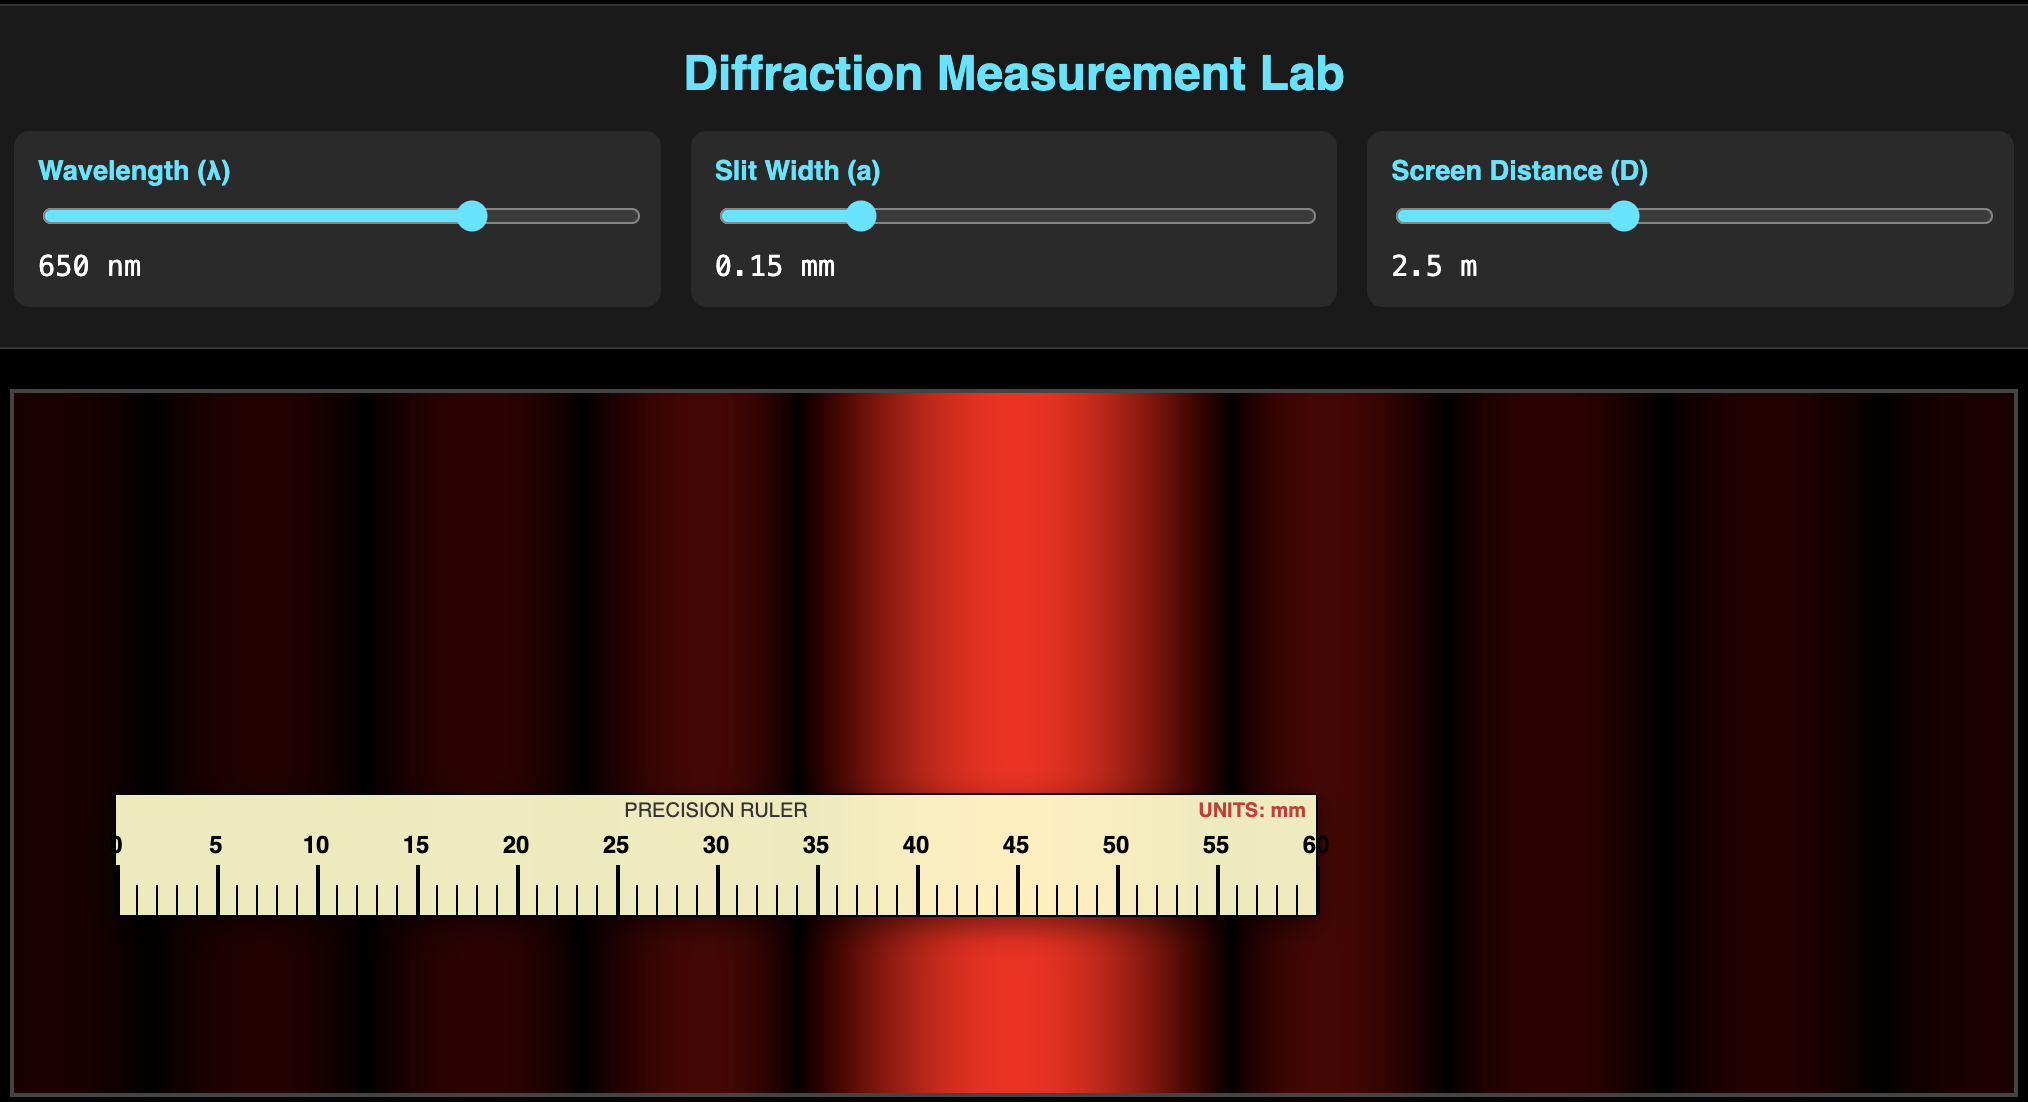
\includegraphics[width=0.95\linewidth]{../../assets/figures/simulations/figure_diffraction_simulation_interface.png}
\caption{Grade 10 single-slit diffraction simulation interface showing slider-controlled wavelength, slit width, and screen distance together with the visual diffraction pattern and measurement support.}
\label{fig:diffraction_interface}
\end{figure}

The initial AI-generated prototype successfully reproduced the general diffraction pattern but required substantial refinement before classroom deployment. Early versions suffered from limited fringe visibility, unrealistic scaling behavior, and insufficient measurement precision for use as a laboratory activity. As a result, the development process shifted from simply producing a visual demonstration to constructing a classroom-oriented virtual experiment.

One major refinement involved improving the visibility of secondary diffraction fringes. The original intensity distribution caused higher-order fringes to become too dim for reliable observation when projected in a classroom setting. To address this issue, brightness scaling and gamma-style visual enhancement were introduced to increase contrast while preserving the overall diffraction structure. This adjustment improved student ability to distinguish fringe boundaries and identify the central maximum during measurement tasks.

A second major pedagogical modification involved the addition of a calibrated on-screen ruler. The initial simulation allowed students to observe pattern changes qualitatively, but it did not support quantitative measurement. A digital ruler overlay was therefore incorporated so that students could measure the width of the central maximum directly on the screen. This transformed the activity from a passive visualization into an interactive virtual laboratory in which students could compare measured values against theoretical predictions based on diffraction relationships.

The simulation also required repeated adjustments to scaling and zoom behavior. In early versions, some parameter combinations generated patterns that were either too compressed to measure accurately or too wide to remain visible on the display window. The zoom and parameter ranges were therefore constrained to maintain observable fringe structures across the intended classroom operating range. These modifications ensured that students could perform measurements consistently without losing the physical relationship between the variables.

Alongside the simulation itself, a companion digital worksheet was developed using fillable \LaTeX{} forms. The worksheet guided students through prediction, observation, measurement, and comparison tasks while integrating simple error-analysis exercises. Students were asked to record measured fringe widths, compare them with expected trends, and explain how changing physical variables altered the diffraction pattern. The worksheet therefore functioned as a structured inquiry tool rather than merely a record sheet.

The complete activity was tested locally on classroom systems before deployment. During this phase, practical deployment issues emerged, including file-format compatibility problems associated with macOS TextEdit saving HTML files in rich-text format. Additional instructions were added to ensure that simulations could be reliably executed in standard web browsers during classroom use.


Overall, the Grade 10 diffraction case study demonstrated that the teacher-guided AI-assisted workflow could evolve from a technically functional visualization into a curriculum-aligned virtual laboratory through iterative refinement, pedagogical filtering, and classroom-oriented testing.

\section{Case Study 2: Grade 12 Transformer and LCR Simulations}

The second classroom case study involved the development of virtual laboratory activities for Grade 12 Physics, covering transformer behaviour and series LCR circuits. In contrast with the Grade 10 diffraction case, which required several rounds of refinement to establish a usable classroom format, the Grade 12 simulations were developed after the earlier interaction had already established a preferred design pattern for virtual laboratory tools. The teacher's prompts were therefore shorter and more operational, asking the AI system to create simulations in which transformer output voltage changed with primary and secondary turns, and in which LCR circuit quantities could be varied and observed in real time.

For the transformer activity, the simulation used the ideal transformer relation as the central model,
\begin{equation}
\frac{V_s}{V_p}=\frac{N_s}{N_p},
\end{equation}
where $V_p$ and $V_s$ represent the primary and secondary voltages, and $N_p$ and $N_s$ represent the number of turns in the primary and secondary coils. The interface allowed students to vary input voltage and turn numbers using range sliders, while numerical voltage displays updated immediately. The simulation also classified the configuration dynamically as step-up, step-down, or approximately equal-voltage, helping students connect numerical ratios with practical transformer categories.

A key visual feature of the transformer simulation was an HTML5 canvas representation of the core and coils. The primary and secondary coils were drawn on opposite sides of the core, with apparent turn density changing in response to the selected values of $N_p$ and $N_s$. A simple animated magnetic-flux representation used moving visual markers inside the core to indicate that changing magnetic flux links the two coils. Although the animation was not intended as a quantitative flux model, it provided a useful conceptual bridge between the transformer equation and Faraday's law of induction.

\begin{figure}[htbp]
\centering
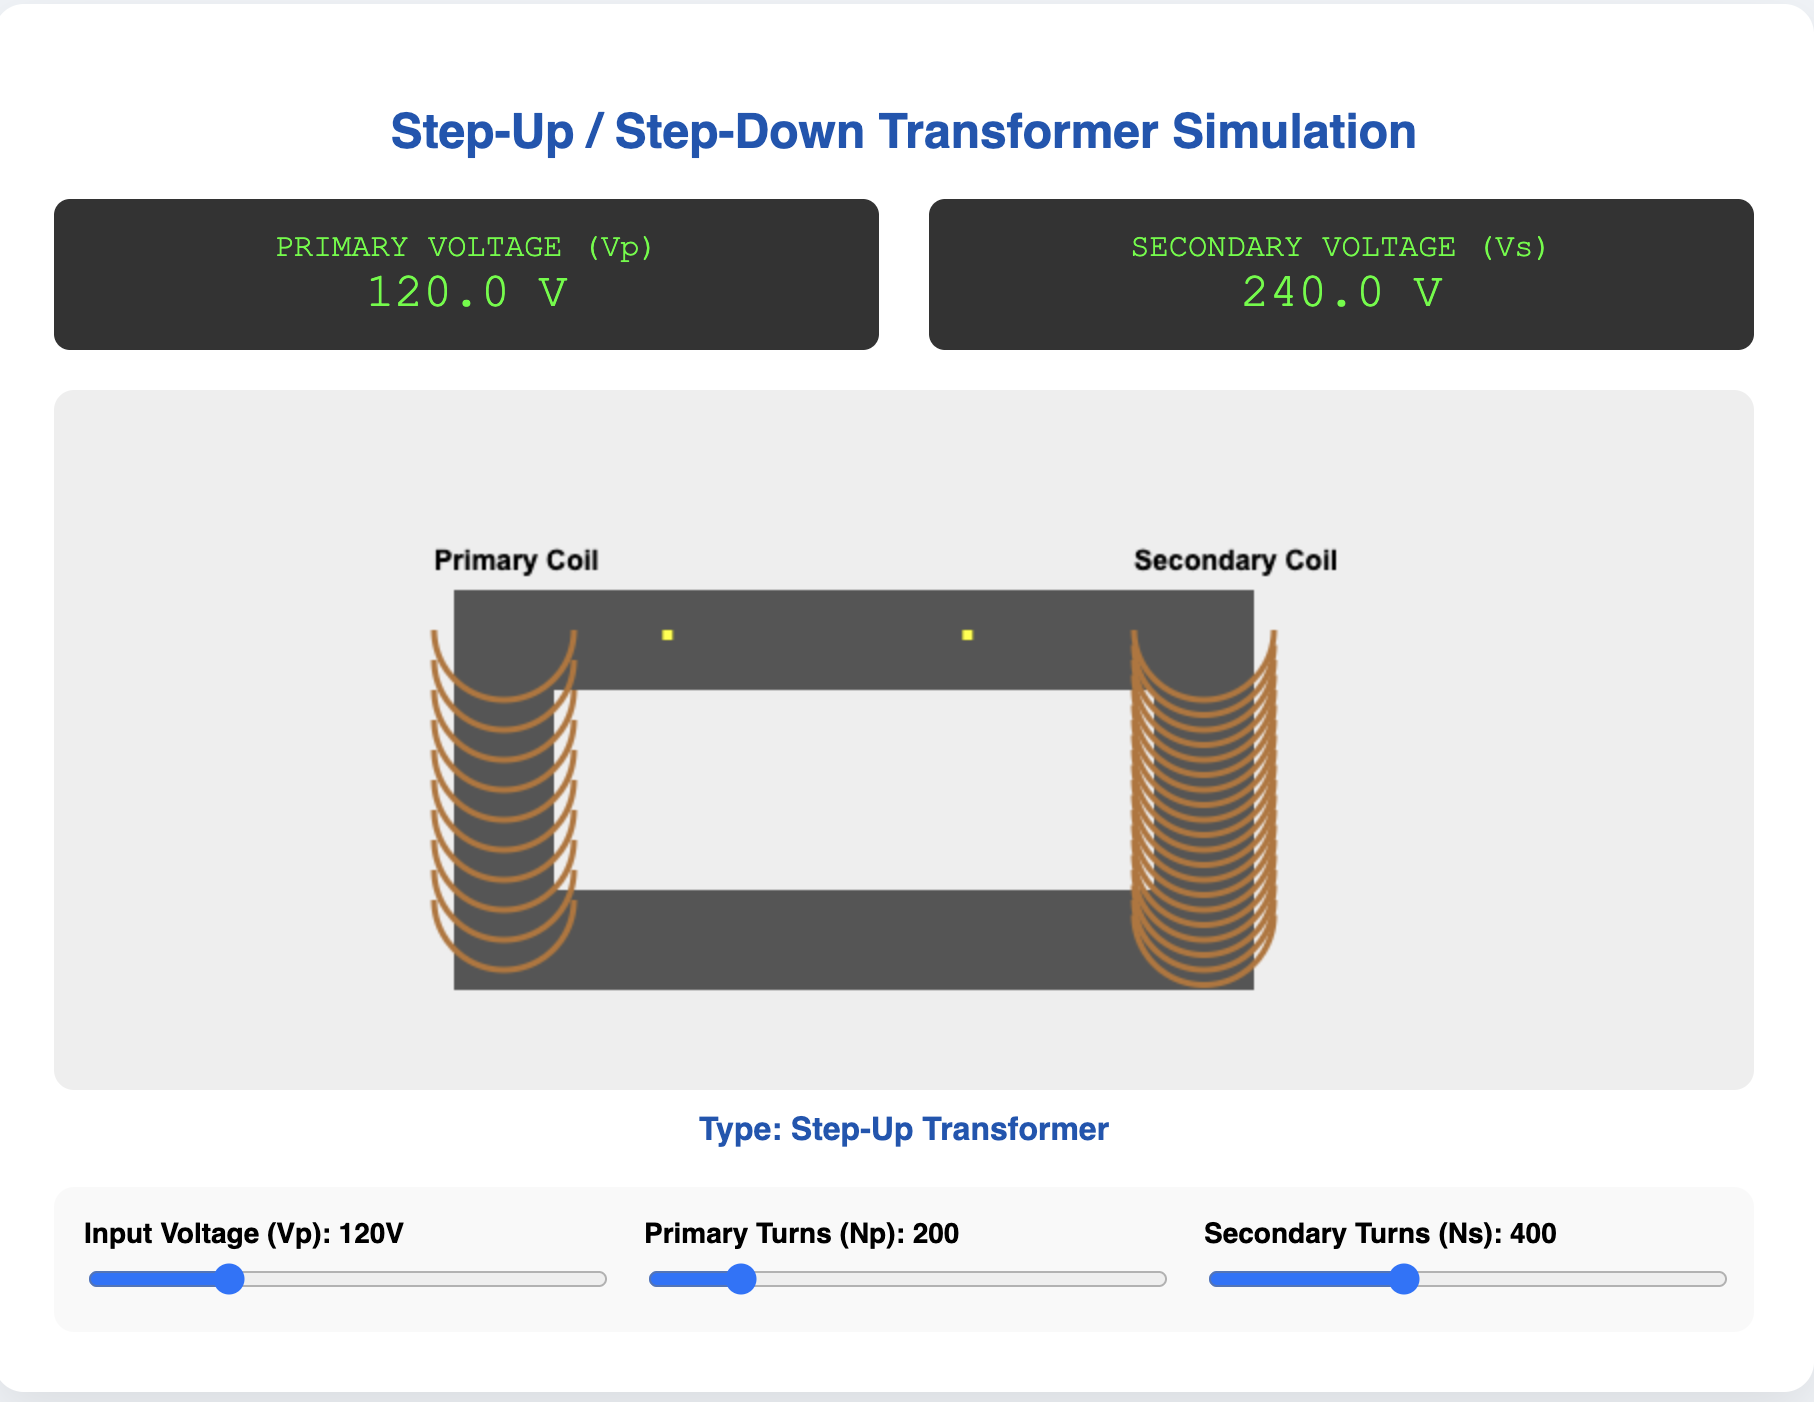
\includegraphics[width=0.95\linewidth]{../../assets/figures/simulations/figure_transformer_simulation_interface.png}
\caption{Grade 12 transformer simulation interface showing live primary and secondary voltage readouts, turn-number controls, and a canvas-based transformer core and coil representation.}
\label{fig:transformer_interface}
\end{figure}

The companion transformer worksheet was produced using fillable \LaTeX{} fields. Students recorded $V_p$, $N_p$, $N_s$, simulated $V_s$, and calculated theoretical $V_s$, allowing direct comparison with the ideal transformer law. The worksheet then extended the task beyond voltage ratios by introducing power, energy, and efficiency analysis. Students calculated input power, output power, percentage efficiency, and energy loss over a specified time interval using
\begin{equation}
\eta = \frac{P_{\mathrm{out}}}{P_{\mathrm{in}}}\times 100\% .
\end{equation}
This extension connected the ideal transformer relationship to more realistic discussions of heating, losses, and non-ideal energy transfer.

The series LCR activity followed the same warm-start design logic. The simulation allowed students to vary circuit parameters such as resistance, inductance, capacitance, and frequency, while observing their effects on inductive reactance, capacitive reactance, impedance, and current. The central relationships were, with $\omega=2\pi f$ as the angular frequency,
\begin{equation}
X_L=\omega L, \qquad X_C=\frac{1}{\omega C}, \qquad Z=\sqrt{R^2+(X_L-X_C)^2}.
\end{equation}
Real-time numerical displays functioned like digital meters, helping students connect changes in circuit parameters with observable AC circuit behaviour. The accompanying worksheet guided students to compare calculated and simulated values, identify resonance-related trends, and interpret how the balance between $X_L$ and $X_C$ affects total impedance.

\begin{figure}[htbp]
\centering
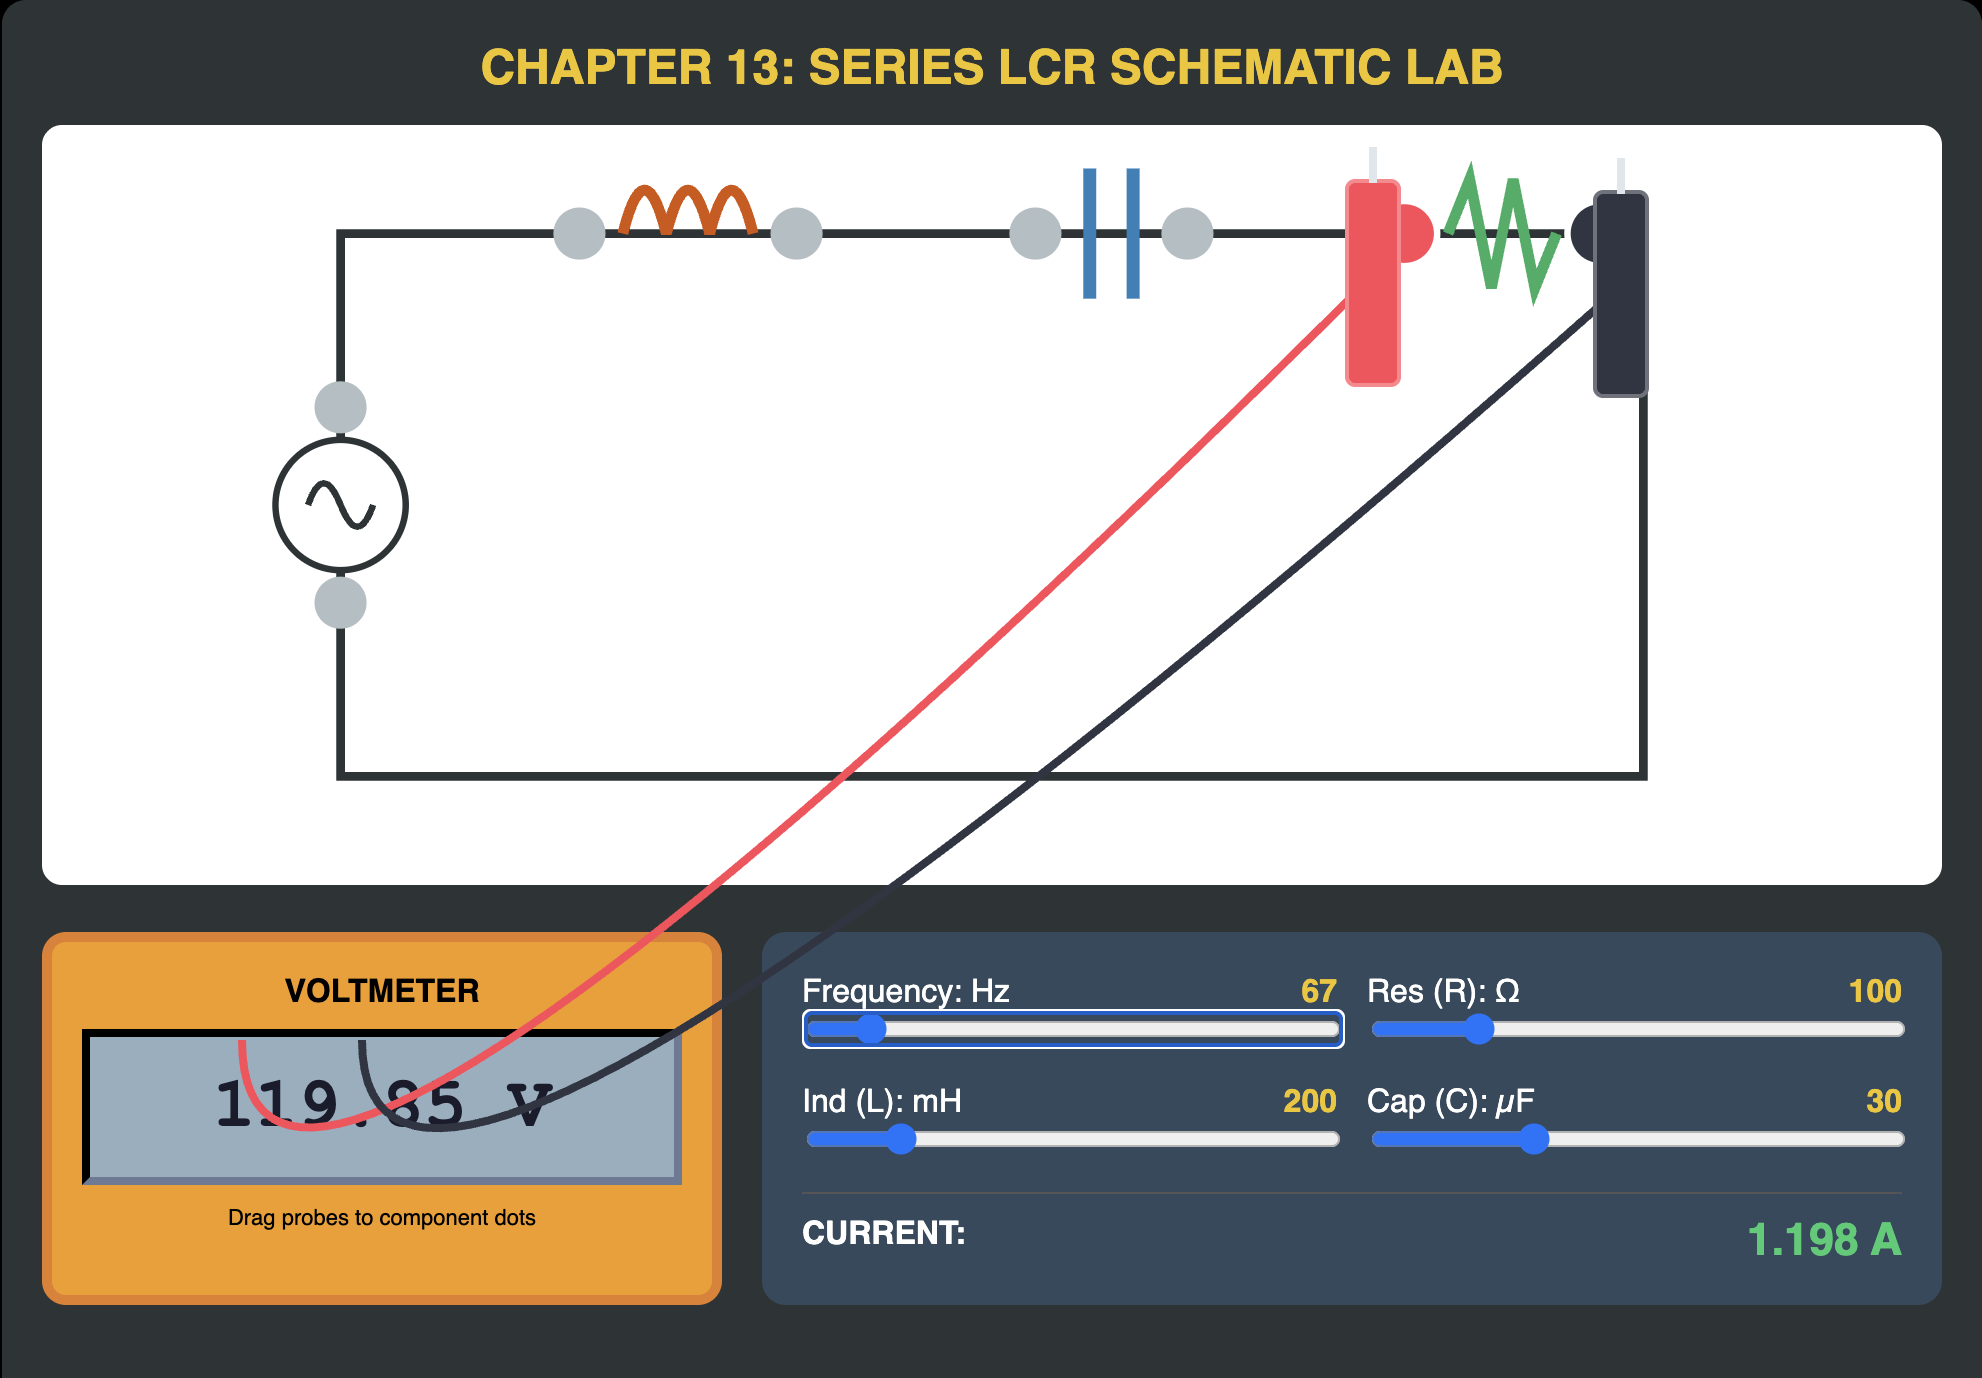
\includegraphics[width=0.95\linewidth]{../../assets/figures/simulations/figure_lcr_simulation_interface.png}
\caption{Grade 12 series LCR circuit simulation interface showing adjustable resistance, inductance, capacitance, and frequency controls together with real-time digital meter displays.}
\label{fig:lcr_interface}
\end{figure}


Taken together, the transformer and LCR activities served as warm-start examples within the broader teacher--AI co-development process. Because interface expectations, worksheet format, and classroom usability preferences had already been established during the diffraction case, the Grade 12 tools required fewer corrective turns before becoming usable. This suggested that sustained conversational context could support continuity of design style across multiple physics topics, while the teacher still remained responsible for checking the physical interpretation, parameter ranges, and classroom suitability of the generated materials.

\section{Classroom Feedback}

After classroom use, exploratory student feedback was collected using a short generic survey on AI-assisted physics simulations and digital laboratory activities. The survey questions were not topic-specific: Grade 10 students responded after using the diffraction activity, while Grade 12 students responded after using the transformer and LCR activities. For this reason, the feedback is interpreted as evidence of student perception of the broader AI-assisted virtual-laboratory approach, rather than as a controlled measure of learning gain for any one physics topic.

A total of 19 student responses were available for analysis. The responses indicated generally positive perceptions of the digital laboratory activities. Students rated the visual representation of physics concepts highly, with an approximate mean score of 4.42 on a five-point scale. Engagement and interest were also rated positively, with an approximate mean score of 4.37. Usability-related items received similarly favourable responses, with an approximate mean score of 4.26. Items related to experimental understanding and confidence were also positive, generally falling between 4.16 and 4.37 on the same scale.

\begin{table}[htbp]
\caption{Summary of exploratory student feedback on the AI-assisted virtual laboratory activities. Scores are reported on a five-point scale and are interpreted descriptively only.}
\label{tab:student_feedback}
\centering
\begin{tabular}{p{5.5cm} p{3.0cm} p{4.5cm}}
\hline
\textbf{Feedback area} & \textbf{Approximate mean score} & \textbf{Interpretation} \\
\hline
Visual representation of physics concepts & 4.42 & Strongly positive perception of visual clarity \\
Interest and engagement & 4.37 & Students generally found the activities engaging \\
Ease of use and usability & 4.26 & Students generally found the simulations manageable to use \\
Experimental understanding and confidence & 4.16--4.37 & Positive perceived support for measurement and interpretation \\
\hline
\end{tabular}
\end{table}


In addition to the post-activity survey, brief in-class polls were conducted with the Grade 12 cohort immediately after the transformer activity. These polls provided more topic-specific feedback on the transformer simulation. All responding students rated the simulation as very easy to use, indicating that they needed no help during the activity. In a separate item on transformer efficiency, 75\% of respondents strongly agreed that the simulation helped them understand why real transformers are less than 100\% efficient, while 25\% selected a neutral response. When asked which simulation feature was most helpful, 75\% selected the visual comparison of primary and secondary coils, while 25\% selected the live voltage readouts. Although these polls were informal and involved only the small Grade 12 class group, they provided useful triangulation with the broader survey findings, particularly regarding usability, visual interpretation, and perceived conceptual support.

Open-ended comments provided additional classroom insight. Several students referred to the usefulness of changing variables and immediately observing the effect on the simulation output. Others highlighted the visual nature of the activities, especially the ability to see relationships that are difficult to observe directly in a normal classroom setting. In the diffraction activity, the measurement component helped connect a visual pattern with calculation and error analysis. In the Grade 12 activities, the real-time numerical displays helped students connect changing circuit or transformer parameters with the corresponding physical quantities.

The feedback should be read cautiously because the sample size was small and because the survey instrument was designed for practical classroom reflection rather than formal psychometric evaluation. In addition, the Grade 10 and Grade 12 responses relate to different simulations. Nevertheless, the results suggest that students perceived the AI-assisted virtual laboratories as visually clear, usable, and supportive of experimental understanding. These findings are consistent with the purpose of the project: not to replace physical laboratory work, but to provide teacher-adapted digital environments that make abstract relationships easier to manipulate, measure, and discuss.

\section{Discussion}

The two classroom cases suggest that generative AI can function as a practical development partner for physics teachers when its outputs are embedded within an active teacher-led design cycle. The central contribution of the workflow was not that the AI system independently produced complete classroom resources, but that it accelerated the production of editable prototypes which the teacher could test, critique, and reshape for specific learners, topics, and classroom constraints.

The Grade 10 diffraction case illustrates the importance of iterative refinement. The first versions of the simulation were technically useful but not yet suitable as a classroom laboratory. Teacher feedback transformed the output from a qualitative visualization into a measurement-based activity by adding enhanced fringe visibility, calibrated ruler tools, controlled parameter ranges, and a structured worksheet. This shows that AI-generated simulations may require substantial pedagogical filtering before they become usable teaching resources.

The Grade 12 transformer and LCR cases show a different feature of the workflow: domain flexibility. Once a design pattern had been established through the diffraction case, similar interface structures could be transferred to new physics topics using much shorter prompts. The later simulations reused familiar elements such as sliders, numerical readouts, canvas-based visualizations, and fillable worksheets, but applied them to different physical relationships. This efficiency gain may be partly attributable to the sustained conversational context: because the transformer and LCR simulations were requested within the same chat thread as the diffraction tool, the AI appeared to retain and apply design preferences established during the earlier exchanges. This suggests that teacher-guided AI development may be especially useful for producing families of related classroom tools rather than isolated one-off resources.

The cases also highlight a form of replicability that is practical rather than statistical. The workflow can be summarized as: state the classroom objective, request a working prototype, test it locally, identify scientific or pedagogical weaknesses, refine the prompt, and repeat until the tool supports the intended lesson. Other teachers may not reproduce the exact simulations described here, but they can adapt the same process to topics such as waves, circuits, mechanics, or optics. The key transferable element is the teacher's role as designer, verifier, and classroom adapter.

At the same time, the study shows clear limitations. AI-generated code should not be treated as automatically correct, especially in physics education where inappropriate parameter ranges, misleading visual scaling, or incorrect assumptions can distort the intended concept. The teacher must check the physics model, classroom usability, and assessment alignment. The student feedback reported here is also exploratory: the sample was small, the survey was generic, and the Grade 10 and Grade 12 students used different simulations. Therefore, the findings should be interpreted as classroom evidence of usability and perceived value, not as proof of improved learning outcomes.

Overall, the cases support a cautious but constructive view of AI-assisted instructional development. Generative AI can reduce the technical barrier to creating custom simulations and worksheets, but its educational value depends on sustained teacher judgement. In this workflow, AI acted as a coding and formatting accelerator, while the teacher remained responsible for deciding what was scientifically valid, pedagogically useful, and practically deployable in the classroom. For physics teachers considering similar approaches, the key recommendation is to begin with a familiar topic, expect to invest several rounds of refinement in the first tool, and then leverage the established design pattern for subsequent simulations in other topic areas.

\section{Conclusion}

This classroom case study illustrates how generative AI can support the rapid development of curriculum-linked virtual physics laboratories when embedded within a teacher-led refinement process. The diffraction case showed the importance of iterative pedagogical correction, while the transformer and LCR cases suggested that established design patterns can be reused across topics. The findings should be interpreted as exploratory classroom evidence rather than proof of learning gains, but they indicate that students perceived the tools as usable, engaging, and helpful for visualizing abstract physics relationships. The central implication is that AI can assist physics teachers in creating adaptable digital laboratories, provided that the teacher remains responsible for scientific verification, classroom fit, and final instructional judgement.

\ack{The author thanks the students who participated in the classroom activities and provided feedback on the digital laboratory tools. The author also acknowledges the support of Khalifa Bin Zayed School and the Ministry of Education, United Arab Emirates, for providing the teaching context in which these classroom activities were developed and implemented.}

\funding{This work received no external funding.}
% This section is a list of funder names and grant numbers

\roles{Anurag Garg: conceptualization, methodology, software development supervision, classroom implementation, data collection, analysis, writing--original draft, and writing--review and editing.}
% List author names and the contributions made to the article, using terms from the NISO Contributor Roles Taxonomy (CRediT) https://credit.niso.org

\data{The classroom materials, simulation files, worksheets, manuscript sources, and supporting documentation are available at: https://github.com/mranuraggarg/teacher-guided-ai-virtual-physics-labs}
% For more information on IOP Publishing's research data policy see: https://publishingsupport.iopscience.iop.org/questions/research-data/

\suppdata{No separate supplementary data files are submitted with this manuscript. Supporting materials are available through the GitHub repository listed in the data availability statement.}




\section*{References}

\begin{thebibliography}{99}

\bibitem{finkelstein2006}
Finkelstein N, Adams W, Keller C, Perkins K and Wieman C 2006 High-Tech Tools for Teaching Physics: The Physics Education Technology Project \textit{Journal of Online Learning and Teaching} \textbf{2}(3)

\bibitem{wieman2010}
Wieman C E, Adams W K, Loeblein P and Perkins K K 2010 Teaching Physics Using PhET Simulations \textit{The Physics Teacher} \textbf{48}(4) 225--227 doi:10.1119/1.3361987

\bibitem{clark2015}
Clark D B, Tanner-Smith E E and Killingsworth S S 2016 Digital Games, Simulations, and Learning: A Systematic Review and Meta-Analysis \textit{Review of Educational Research} \textbf{86}(1) 79--122

\bibitem{rutten2012}
Rutten N, van Joolingen W R and van der Veen J T 2012 The learning effects of computer simulations in science education \textit{Computers \& Education} \textbf{58}(1) 136--153 doi:10.1016/j.compedu.2011.07.017

\bibitem{smetana2012}
Smetana L K and Bell R L 2011 Computer Simulations to Support Science Instruction and Learning: A critical review of the literature \textit{International Journal of Science Education} \textbf{34}(9) 1337--1370 doi:10.1080/09500693.2011.605182

\bibitem{banda2021}
Banda H J and Nzabahimana J 2021 Effect of integrating physics education technology simulations on students' conceptual understanding in physics: A review of literature \textit{Physical Review Physics Education Research} \textbf{17}(2) 023108 doi:10.1103/PhysRevPhysEducRes.17.023108

\bibitem{sellberg2026}
Sellberg C and Lindwall O 2025 Simulation-based training in professional education: learning, participation, and instructional design \textit{Instructional Science} \textbf{54} 9 doi:10.1007/s11251-025-09763-2

\bibitem{holmes2022}
Holmes W and Tuomi I 2022 State of the Art and Practice in AI in Education \textit{European Journal of Education} \textbf{57}(4) 542--570 doi:10.1111/ejed.12533

\bibitem{celik2022}
Celik I, Dindar M, Muukkonen H and J{\"a}rvel{\"a} S 2022 The Promises and Challenges of Artificial Intelligence for Teachers: A Systematic Review of Research \textit{TechTrends} \textbf{66}(4) 616--630 doi:10.1007/s11528-022-00715-y

\bibitem{hodges2024}
Hodges C B and Kirschner P A 2023 Innovation of Instructional Design and Assessment in the Age of Generative Artificial Intelligence \textit{TechTrends} \textbf{68} 195--199 doi:10.1007/s11528-023-00926-x

\bibitem{li2024}
Li Y, Keung J and Ma X 2024 Integrating Generative AI in Software Engineering Education: Practical Strategies \textit{2024 International Symposium on Educational Technology (ISET)} pp 49--53 doi:10.1109/ISET61814.2024.00019

\bibitem{baidoo2025}
Baidoo-Anu D and Owusu Ansah L 2023 Education in the Era of Generative Artificial Intelligence (AI): Understanding the Potential Benefits of ChatGPT in Promoting Teaching and Learning \textit{Journal of AI} \textbf{7}(1) 52--62 doi:10.61969/jai.1337500

\bibitem{huang2026}
Huang T, Ren Z, Huang Y et al. 2026 Hallucination detection in LLM code generation: A sampling-based consensus verification approach \textit{Automated Software Engineering} \textbf{33} 70 doi:10.1007/s10515-026-00605-0

\bibitem{techreport2023}
United States Office of Educational Technology 2023 \textit{Artificial Intelligence and the Future of Teaching and Learning: Insights and Recommendations} (Washington, DC: U.S. Department of Education) Available at: https://digital.library.unt.edu/ark:/67531/metadc2114121/

\bibitem{xing2025}
Xing Z, Liu Y, Cheng Z, Huang Q, Zhao D, Sun D and Liu C 2025 When Prompt Engineering Meets Software Engineering: CNL-P as Natural and Robust ``APIs'' for Human-AI Interaction \textit{arXiv preprint} arXiv:2508.06942 [cs.SE] doi:10.48550/arXiv.2508.06942


\bibitem{brown2020}
Brown T B, Mann B, Ryder N, Subbiah M, Kaplan J, Dhariwal P, Neelakantan A, Shyam P, Sastry G \textit{et al.} 2020 Language Models are Few-Shot Learners \textit{arXiv preprint} arXiv:2005.14165 [cs.CL] doi:10.48550/arXiv.2005.14165

\bibitem{lazaros2026}
Lazaros K, Vrahatis AG, Kotsiantis S. Human-in-the-Loop Artificial Intelligence: A Systematic Review of Concepts, Methods, and Applications. Entropy. 2026; 28(4):377. doi:10.3390/e28040377

\bibitem{schmager2025}
Schmager S, Pappas I O and Vassilakopoulou P 2025 Understanding Human-Centred AI: a review of its defining elements and a research agenda \textit{Behaviour \& Information Technology} \textbf{44}(15) 3771--3810 doi:10.1080/0144929X.2024.2448719

\bibitem{liu2026}
Liu F, Liu Y, Shi L, Yang Z, Zhang L, Lian X, Li Z and Ma Y 2026 Beyond Functional Correctness: Exploring Hallucinations in LLM-Generated Code \textit{arXiv preprint} arXiv:2404.00971 [cs.SE] doi:10.48550/arXiv.2404.00971

\end{thebibliography}



\end{document}
